\newpage
\begin{figure}
    \begin{center}
        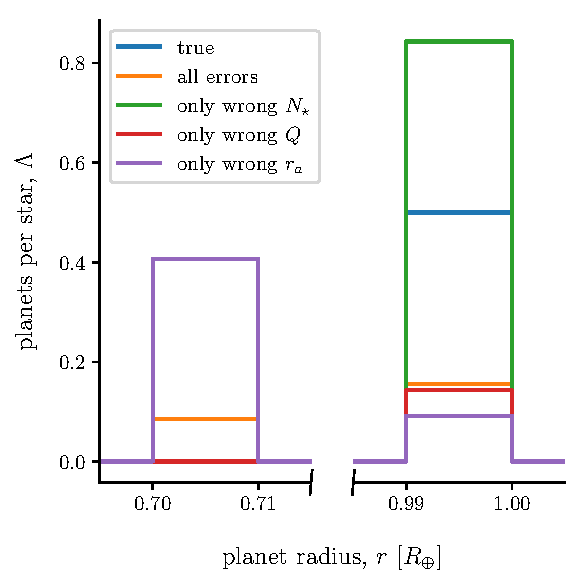
\includegraphics[width=\textwidth]{figures/errcases_rate_density_vs_radius_model_1_brokenx.pdf}
    \end{center}
    \caption{
    Inferred planet occurrence rates as a function of planet radius in Model 
    \#1.
    This model has fixed stars, fixed planets, and twin binaries.
    If the true planet radius is $r_p$, all planets 
    detected in binaries will have apparent radii $r_a = r_p/\sqrt{2}$.
    Only 1 in 8 selected binaries is actually searchable (see 
    Sec.~\ref{sec:model_1}).
    To help illustrate the individual effects of errors, we 
    separated them:
    ``only wrong $N_\star$'' means the only error is an incorrectly assumed 
    number of selected stars;
    ``only wrong $Q$'' means the only error is an incorrectly assumed 
    detection efficiency (including both miscalculated transit probabilities 
    and 
    fraction of selected stars that are searchable);
    ``only wrong $r_a$'' means the only error is misinterpretation of 
    planetary radii, due to both transit depth dilution and also wrongly 
    assumed host star radii.
    }
    \label{fig:errcases_model_1}
\end{figure}

\begin{figure}[!tb]
    \centering
    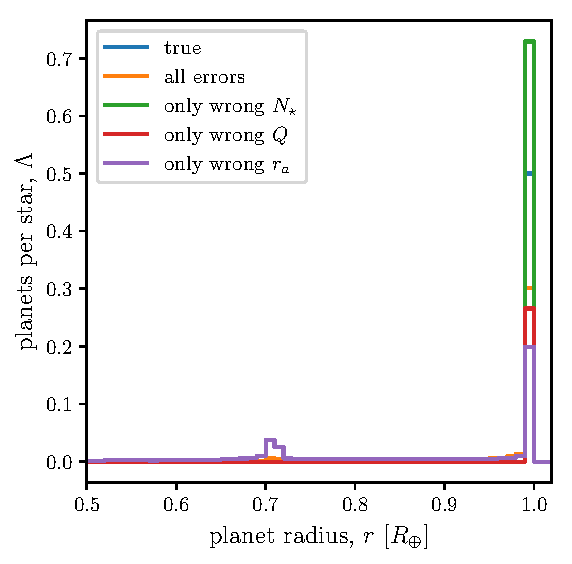
\includegraphics[width=.7\textwidth]{figures/errcases_rate_density_vs_radius_model_2.pdf}
    %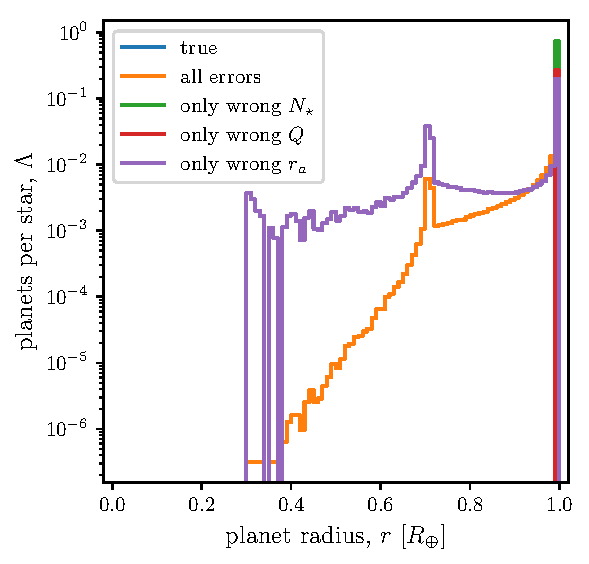
\includegraphics[width=1.0\textwidth]{figures/errcases_rate_density_vs_radius_logs_model_2.pdf}
    \caption{
    Inferred planet occurrence rates as a function of planet radius in Model 
    \#2.
    This model has fixed planets and primaries, but varying secondaries.
    }
    \label{fig:errcases_model_2_linear}
\end{figure}

\begin{figure}[!tb]
    \centering
    %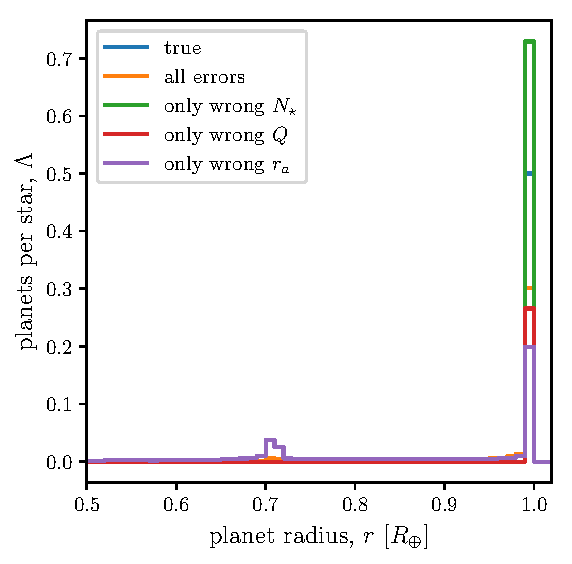
\includegraphics[width=1.0\textwidth]{figures/errcases_rate_density_vs_radius_model_2.pdf}
    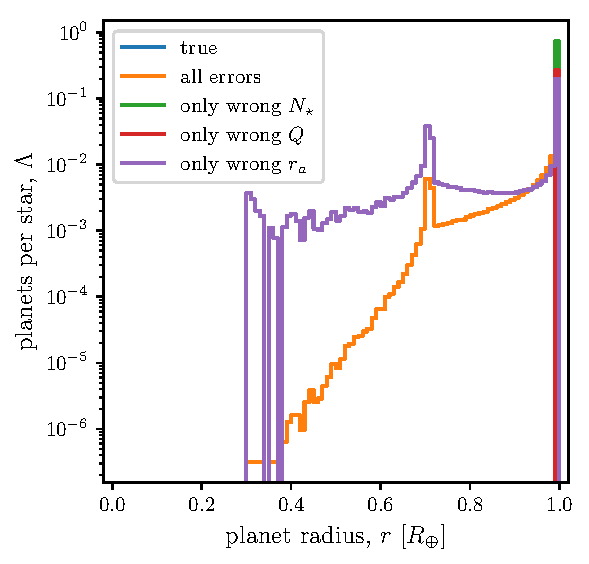
\includegraphics[width=.7\textwidth]{figures/errcases_rate_density_vs_radius_logs_model_2.pdf}
    \caption{
    Same as Fig.~\ref{fig:errcases_model_2_linear}, but with logarithmic 
    $y$-axis, and different $x$ scale.
    }
    \label{fig:errcases_model_2_log}
\end{figure}

\begin{figure}[!tb]
    \centering
    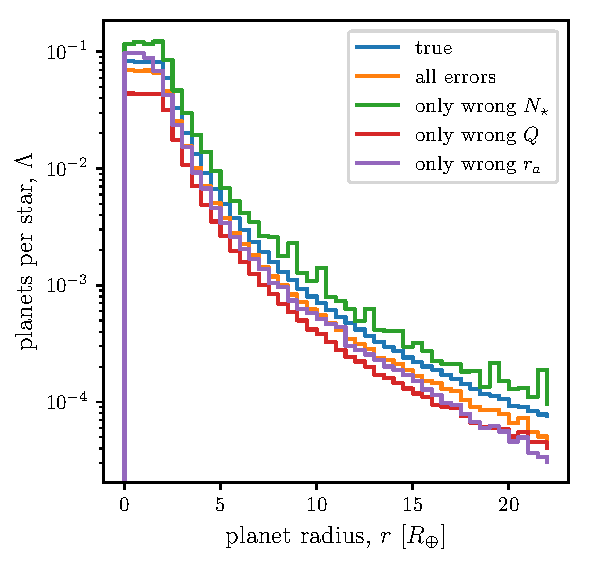
\includegraphics[width=\textwidth]{figures/errcases_rate_density_vs_radius_logs_model_3.pdf}
    \caption{
    Inferred planet occurrence rates as a function of planet radius in Model 
    \#3.
    This model has fixed primaries and single stars, but varying 
    secondaries.
    The true planet radius distribution is a power law with exponent $-2.92$ 
    above $2R_\oplus$, below which it is uniform (e.g., Howard et al., 
    2012).
    }
    \label{fig:errcases_model_3_log}
\end{figure}

\begin{figure}[!tb]
    \centering
    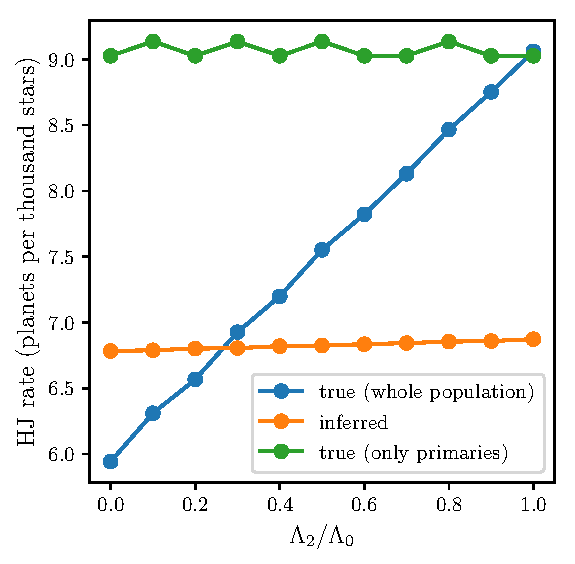
\includegraphics[width=.9\textwidth]{figures/HJ_correction_inputrate_vs_HJratevalues.pdf}
    \caption{
    $\Lambda_i$ is the occurrence rate integrated over all possible phase 
    space for the $i^{\rm th}$ system type. $\Lambda_2/\Lambda_0=1$ 
    corresponds to an equal number of planets per secondary as per single star;
    $\Lambda_2/\Lambda_0=0$ corresponds to secondaries not having any planets.
    In our Model \#3, though the true HJ occurrence rate 
    (Eq.~\ref{eq:occ_rate}) is highly dependent on $\Lambda_2$, 
    the inferred rate hardly depends on whether secondaries have HJs.
    This means that the ``correction factor'' between the inferred rate and 
    the true rate around single stars is underestimated by a factor of 
    $\sim1.3$, independent of the HJ rate around secondaries.
    }
    \label{fig:HJ_correction_inputrate_vs_HJratevalues}
\end{figure}


%\begin{figure}[!b]
%    \begin{center}
%        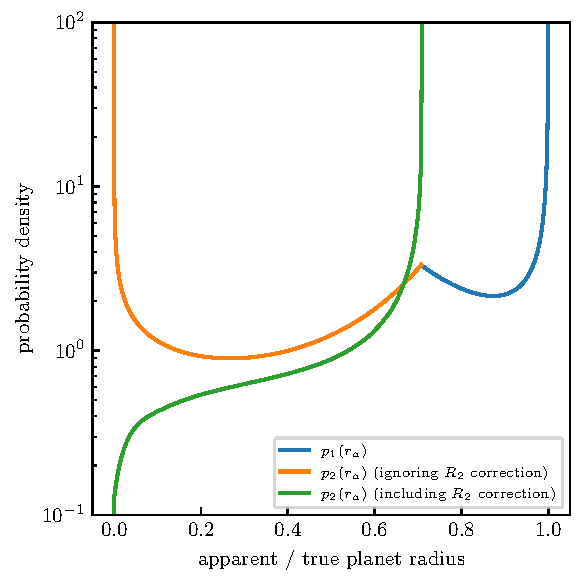
\includegraphics[width=.9\textwidth]{figures/prob_r_a.pdf}
%    \end{center}
%    \caption{Model \#2 (Sec.~\ref{sec:model_2}): 
%    probability of observing an apparent radius $r_a$ given a 
%    planet orbiting the primary, $p_1(r_a)$, or the secondary, $p_2(r_a)$ of 
%    a 
%    binary system.
%    The true planet radius is fixed~--~a delta function centered on ``1''.
%    This plot takes $\alpha=3.5, \beta=0$, for $\alpha$ the exponent in 
%    the mass-luminosity relation $L \propto M^\alpha$, and $\beta$ the 
%    exponent in the distribution of mass ratios in a volume-limited sample.
%    Each distribution is separately normalized.
%    }
%    \label{fig:model2_prob_r_a}
%\end{figure}